\documentclass[11pt,letterpaper,boxed]{hmcpset}
\usepackage[margin=1in]{geometry}
\usepackage{graphicx}
\usepackage{enumerate}
\usepackage{amsmath}
\usepackage{mathtools}
\usepackage{amssymb}
\usepackage{cancel}

\setlength{\parskip}{6pt}
\setlength{\parindent}{0pt}

% convenient delimiters
\newcommand{\set}[1]{\ensuremath{ \left\{ #1 \right\} }}
\newcommand{\pn}[1]{\left( #1 \right)}
\newcommand{\abs}[1]{\left| #1 \right|}
\newcommand{\bk}[1]{\left[ #1 \right]}
\newcommand{\vc}[1]{\left\langle #1 \right\rangle}

% set numbering style for enumerated lists to be of form (a), (b), (c), etc.
\renewcommand{\labelenumi}{{(\alph{enumi})}}


\name{}
\class{Math 35, Section \_\_\_}
\assignment{Problem Set 3}
\duedate{November 10, 2015}


\begin{document} {

    \problemlist{3.\{1.9, 2.15, 2.17, 2.18, 3.32, 3.33\}, 4.\{1.5, 2.13, 3.28(abc), 3.29(abc), 3.30(abc), 3.31, 3.35\}}

%%%%%%%%%%%%%%% Number 1 %%%%%%%%%%%%%%%%%%%%%%%%%%%%%%%%%%%%%%%%%%%%%%%%%

\begin{problem}[3.1.9]
	An individual named Claudius is located at the point 0 in the accompanying diagram.\\
	\begin{center}
		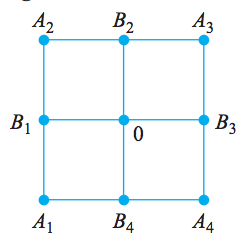
\includegraphics{Nov_10_1.png}
	\end{center}
	Using an appropriate randomization device (such as a tetrahedral die, one having four sides), Claudius first move to one of the four locations $B_1$, $B_2$, $B_3$, $B_4$. Once at one of these locations, another randomization device is used to decide whether Claudius next returns to 0 or next visits one of the other two adjacent points. This process then continues; after each move, another move to one of the (new) adjacent points is determined by tossing an appropriate die or coin.
	\begin{enumerate}
		\item
			Let $X$ = the number of moves that Claudius makes before first returning to 0. What are possible values of $X$? Is $X$ discrete or continuous?
		\item
			If moves are allowed also along the diagonal paths connecting 0 to $A_1$, $A_2$, $A_3$, and $A_4$, respectively answer the questions in part (a).
	\end{enumerate}
\end{problem}

\begin{solution}
	\vfill
\end{solution}
\newpage

%%%%%%%%%%%%%%% Number 2 %%%%%%%%%%%%%%%%%%%%%%%%%%%%%%%%%%%%%%%%%%%%%%%%%

\begin{problem}[3.2.15]
	Many manufacturers have quality control programs that include inspection of incoming materials for defects. Suppose a computer manufacturer receives computer boards in lots of five. Two boards are selected from each lot for inspection. We can represent possible outcomes of the selection process by pairs. For example, the pair (1, 2) represents the selection of boards 1 and 2 for inspection.
	\begin{enumerate}
		\item
			List the ten different possible outcomes.
		\item
			Suppose that boards 1 and 2 are the only defective boards in a lot of five. Two boards are to be chosen at random. Define $X$ to be the number of defective boards observed among those inspected. Find the probability distribution of $X$.
		\item
			Let $F(x)$ denote the cdf of $X$. First determine $F(0) = P(X \leq 0)$, $F(1)$, and $F(2)$; then obtain $F(x)$ for all other $x$.
	\end{enumerate}
\end{problem}

\begin{solution}
	\vfill
\end{solution}
\newpage

%%%%%%%%%%%%%%% Number 3 %%%%%%%%%%%%%%%%%%%%%%%%%%%%%%%%%%%%%%%%%%%%%%%%%

\begin{problem}[3.2.17]
	A new battery's voltage may be acceptable $(A)$ or unacceptable $(U)$. A certain flashlight requires two batteries, so batteries will be independently selected and tested until two acceptable ones have been found. Suppose that 90\% of all batteries have acceptable voltages. Let $Y$ denote the number of batteries that must be tested.
	\begin{enumerate}
		\item
			What is $p(2)$, that is, $P(Y = 2)$?
		\item
			What is $p(3)$? [\textit{Hint}: There are two different outcomes that result in $Y = 3$.]
		\item
			To have $Y = 5$, what must be true of the fifth battery selected? List the four outcomes for which $Y = 5$ and then determine $p(5)$.
		\item
			Use the pattern in your answers for parts (a) - (c) to obtain a general formula for $p(y)$.
	\end{enumerate}
\end{problem}

\begin{solution}
	\vfill
\end{solution}
\newpage

%%%%%%%%%%%%%%% Number 4 %%%%%%%%%%%%%%%%%%%%%%%%%%%%%%%%%%%%%%%%%%%%%%%%%

\begin{problem}[3.2.18]
	Two fair six-sided dice are tossed independently. Let $M$ = the maximum of the two tosses (so $M(1,5) = 5$, $M(3,3) = 3$, etc.).
	\begin{enumerate}
		\item
			What is the pmf of $M$? [\textit{Hint}: First determine $p(1)$, then
$p(2)$, and so on.]
		\item
			Determine the cdf of $M$ and graph it.
	\end{enumerate}
\end{problem}

\begin{solution}
	\vfill
\end{solution}
\newpage

%%%%%%%%%%%%%%% Number 5 %%%%%%%%%%%%%%%%%%%%%%%%%%%%%%%%%%%%%%%%%%%%%%%%%

\begin{problem}[3.3.32]
	A certain brand of upright freezer is available in three different rated capacities: 16 ft$^3$, 18 ft$^3$, and 20 ft$^3$. Let $X$ = the rated capacity of a freezer of this brand sold at a certain store. Suppose that $X$ has pmf
	\begin{center}
		\begin{tabular}{c|c c c}
			x & 16 & 18 & 20\\
 			\hline
 			p(x) & 0.2 & 0.5 & 0.3 \\
	 	\end{tabular}
	\end{center}
	\begin{enumerate}
		\item
            Compute $E\bk{X}$, $E\bk{X^2}$, and $V(X)$.
		\item
			If the price of a freezer having capacity $X$ cubic feet is $70X - 650$, what is the expected price paid by the next customer to buy a freezer?
		\item
			What is the variance of the price paid by the next customer?
		\item
			Suppose that although the rated capacity of a freezer is $X$, the actual capacity is $h(X) = X - .008X^2$. What is the expected actual capacity of the freezer purchased by the next customer?
	\end{enumerate}
\end{problem}

\begin{solution}
	\vfill
\end{solution}
\newpage

%%%%%%%%%%%%%%% Number 6 %%%%%%%%%%%%%%%%%%%%%%%%%%%%%%%%%%%%%%%%%%%%%%%%%

\begin{problem}[3.3.33]
	Let $X$ be a Bernoulli rv with pmf as in Example 3.18.
	\begin{enumerate}
		\item
            Compute $E\bk{X^2}$.
		\item
			Show that $V(X) = p(1-p)$.
		\item
            Compute $E\bk{X^{79}}$.
	\end{enumerate}
\end{problem}

\begin{solution}
	\vfill
\end{solution}
\newpage

%%%%%%%%%%%%%%% Number 7 %%%%%%%%%%%%%%%%%%%%%%%%%%%%%%%%%%%%%%%%%%%%%%%%%

\begin{problem}[4.1.5]
	A college professor never finishes his lecture before the end of the hour and always finishes his lectures within 2 min after the hour. Let $X$ = the time that elapses between the end of the hour and the end of the lecture and suppose the pdf of $X$ is
		$$f(x) = \begin{cases}
			kx^2 & 0 \leq x \leq 2 \\
			0 & \mbox{otherwise}
		\end{cases}$$
	\begin{enumerate}
		\item
			Find the value of $k$ and draw the corresponding density curve. [\textit{Hint}: Total area under the graph of $f(x)$ is 1.]
		\item
			What is the probability that the lecture ends within 1 min of the end of the hour?
		\item
			What is the probability that the lecture continues beyond the hour for between 60 and 90 sec?
		\item
			What is the probability that the lecture continues for at least 90 sec beyond the end of the hour?
	\end{enumerate}
\end{problem}

\begin{solution}
	\vfill
\end{solution}
\newpage

%%%%%%%%%%%%%%% Number 8 %%%%%%%%%%%%%%%%%%%%%%%%%%%%%%%%%%%%%%%%%%%%%%%%%

\begin{problem}[4.2.13]
	Example 4.5 introduced the concept of time headway in traffic flow and proposed a particular distribution for $X$ = the headway between two randomly selected consecutive cars (sec). Suppose that in a different traffic environment, the distribution of time headway has the form
		$$f(x) = \begin{cases}
			\dfrac{k}{x^4} & x > 1 \\
			0 & x \leq 1
		\end{cases}$$
	\begin{enumerate}
		\item
			Determine the value of $k $for which $f(x)$ is a legitimate pdf.
		\item
			Obtain the cumulative distribution function.
		\item
			Use the cdf from (b) to determine the probability that headway exceeds 2 sec and also the probability that headway is between 2 and 3 sec.
		\item
			Obtain the mean value of headway and the standard deviation of headway.
		\item
			What is the probability that headway is within 1 standard deviation of the mean value?
	\end{enumerate}
\end{problem}

\begin{solution}
	\vfill
\end{solution}
\newpage

%%%%%%%%%%%%%%% Number 9 %%%%%%%%%%%%%%%%%%%%%%%%%%%%%%%%%%%%%%%%%%%%%%%%%

\begin{problem}[4.3.28]
	Let $Z$ be a standard normal random variable and calculate the following probabilities, drawing pictures wherever appropriate.
	\begin{enumerate}
		\item
			$P(0 \leq Z \leq 2.17)$
		\item
			$P(0 \leq Z \leq 1)$
		\item
			$P(-2.50 \leq Z \leq 0)$
	\end{enumerate}
\end{problem}

\begin{solution}
	\vfill
\end{solution}
\newpage

%%%%%%%%%%%%%%% Number 10 %%%%%%%%%%%%%%%%%%%%%%%%%%%%%%%%%%%%%%%%%%%%%%%%

\begin{problem}[4.3.29]
	In each case, determine the value of the constant $c$ that makes the probability statement correct.
	\begin{enumerate}
		\item
			$\Phi(c) = 0.9838$
		\item
			$P(0 \leq Z \leq c) = 0.291$
		\item
			$P(c \leq Z) = 0.121$
	\end{enumerate}
\end{problem}

\begin{solution}
	\vfill
\end{solution}
\newpage

%%%%%%%%%%%%%%% Number 11 %%%%%%%%%%%%%%%%%%%%%%%%%%%%%%%%%%%%%%%%%%%%%%%%

\begin{problem}[4.3.30]
	Find the following percentiles for the standard normal distribution.  Interpolate where appropriate.
	\begin{enumerate}
		\item
			91st
		\item
			9th
		\item
			75th
	\end{enumerate}
\end{problem}

\begin{solution}
	\vfill
\end{solution}
\newpage

%%%%%%%%%%%%%%% Number 12 %%%%%%%%%%%%%%%%%%%%%%%%%%%%%%%%%%%%%%%%%%%%%%%%

\begin{problem}[4.3.31]
	Determine $z_\alpha$ for the following:
	\begin{enumerate}
		\item
			$\alpha = 0.0055$
		\item
			$\alpha = 0.09$
		\item
			$\alpha = 0.663$
	\end{enumerate}
\end{problem}

\begin{solution}
	\vfill
\end{solution}
\newpage

%%%%%%%%%%%%%%% Number 13 %%%%%%%%%%%%%%%%%%%%%%%%%%%%%%%%%%%%%%%%%%%%%%%%

\begin{problem}[4.3.35]
	In a road-paving process, asphalt mix is delivered to the hopper of the paver by trucks that haul the material from the batching plant. The article "Modeling of Simultaneously Continuous and Stochastic Construction Activities for Simulation" (\textit{J. of Construction Engr. and Mgmnt}., 2014: 1037-1045) proposed a normal standard distribution with mean value 8.46 min and standard deviation of 0.913 min for the rv $X$ = truck haul time.
	\begin{enumerate}
		\item
			What is the probability that haul time will be at least 10m in? Will exceed 10 min?
		\item
			What is the probability that haul time will exceed 15 min?
		\item
			What is the probability that haul time will be between 8 and 10 min?
		\item
			What value $c$ is such that the interval includes 98\% of all haul times are in the interval from 8.46 - $c$ to 8.46 + $c$?
		\item
			If four haul times are independently selected, what is the probability that at least one of them exceeds 10 min?
	\end{enumerate}
\end{problem}

\begin{solution}
	\vfill
\end{solution}


\end{document}
